\documentclass{beamer}
\usepackage{amsmath}
\usepackage{listings}
\usepackage[danish]{babel}
\usepackage[utf8]{inputenc}

\lstset{language=Haskell,basicstyle=\ttfamily}
\usepackage{beamerthemesplit}
\usetheme{Madrid}

\title{Self-adjusting heaps}
\subtitle{A performance comparison}
\author{Johan Brinch \and Asser Femø}
\date{\today}
\newcommand{\bind}{\texttt{>>=}}
\newcommand{\ret}{\texttt{return}}
\newcommand{\bs}{\texttt{\char`\\}}
\newcommand{\fs}{\char`/}
\newcommand{\at}{\texttt{a}}
\newcommand{\kt}{\texttt{k}}
\newcommand{\mt}{\texttt{k}}
\begin{document}
\lstset{basicstyle=\footnotesize\ttfamily}
%\section*{Introduction}
\begin{frame}
  \titlepage
\end{frame}

\section{The Pairing Heap}

\begin{frame}[fragile]
\frametitle{Pairing Heap}
\tableofcontents
\end{frame}

\subsection{Overview}
\begin{frame}[fragile]
\frametitle{Pairing Heap}

\begin{center}
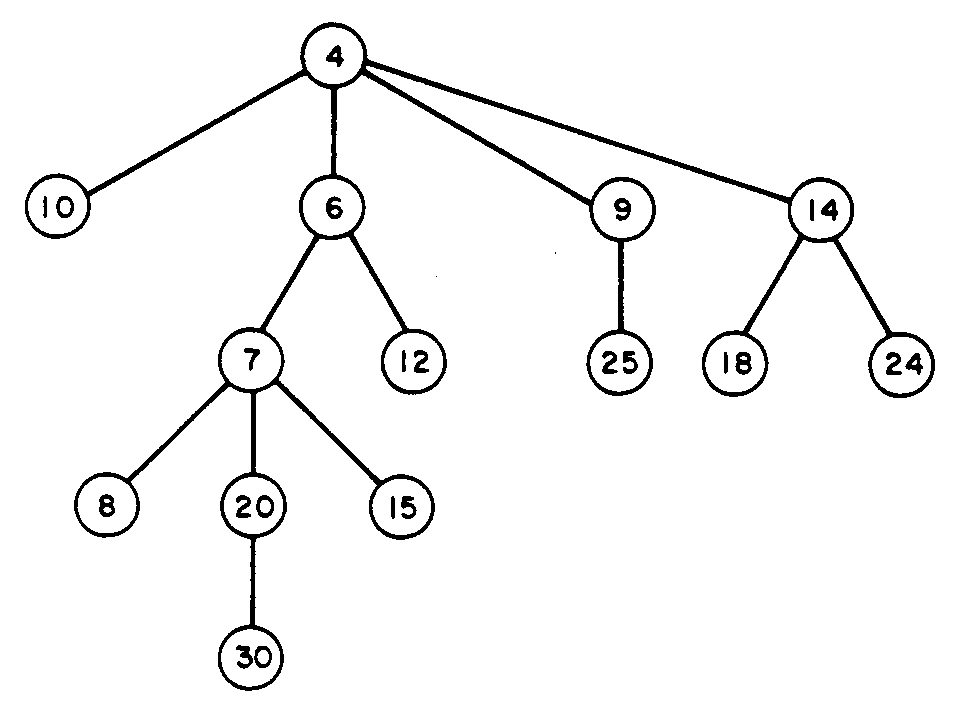
\includegraphics[width=7cm]{../pairing-heap-slides/fig1.png}
\end{center}

\end{frame}

\begin{frame}
\frametitle{Operations}

\begin{description}
\item[link] make the root of smaller key the parent of the root of larger key
\item[insert] make $x$ a single-node tree and link with $H$
\item[delete-min] delete root of $H$, link its children
\item[find-min] return root of $H$
\item[decrease-key] decrease key of $x$, cut $x$ from $H$ and link them
back together
\item[delete] cut $x$ from $H$, do delete-min on $x$ and link its children to $H$
\end{description}

\end{frame}

\begin{frame}
\frametitle{Child-sibling representation}
\begin{center}
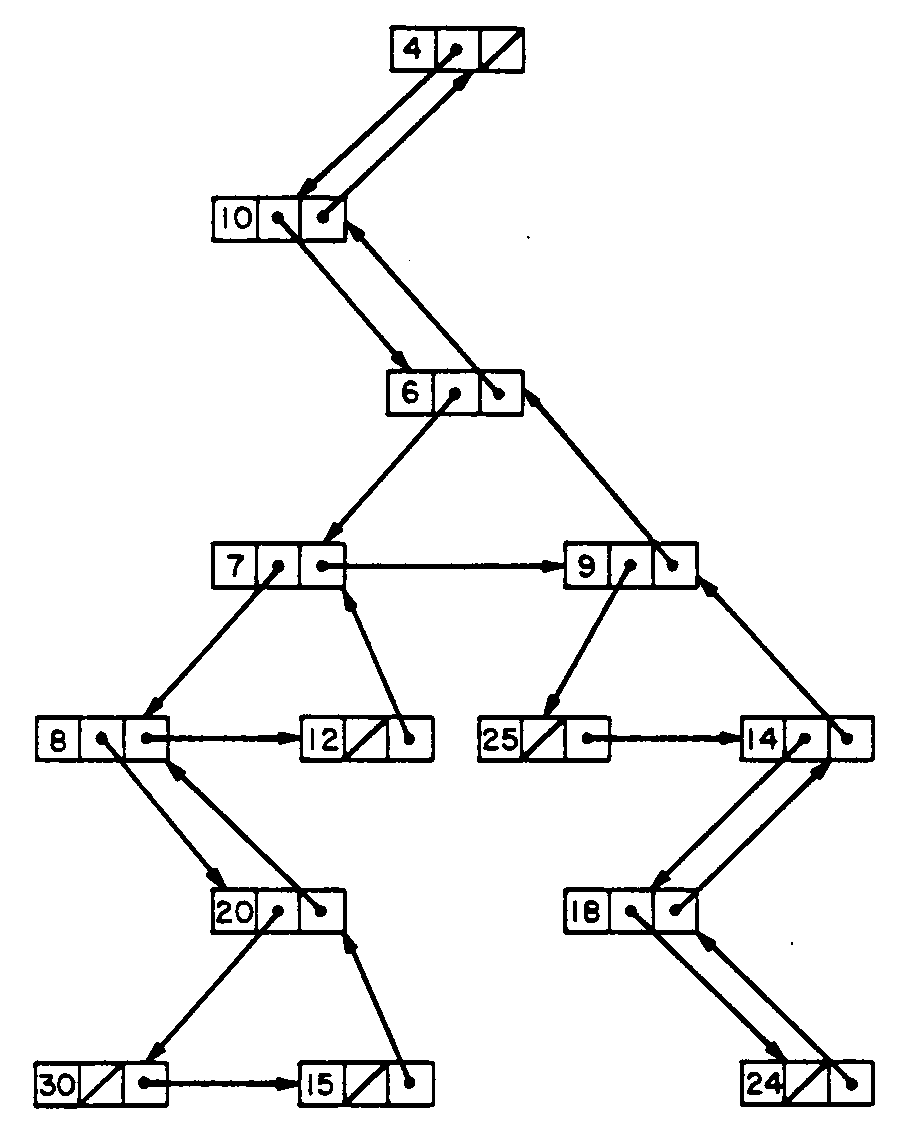
\includegraphics[width=5cm]{../pairing-heap-slides/fig3.png}
\end{center}

\end{frame}

\begin{frame}
\subsection{Running Time}
\frametitle{Running Time}

\begin{itemize}
\item \textbf{find-min}, \textbf{insert}, \textbf{meld} and \textbf{decrease-key}:
  $O(1)$ worst-case time.
\item \textbf{delete-min} and \textbf{delete}: $\Theta(n)$ worst case
  time.\\ Can be improved to $O(\log n)$ amortized time by two-pass or multipass linking.
\end{itemize}

\end{frame}

\begin{frame}
\frametitle{Variations}
\frametitle{Variations}

\textbf{Stasko-Vitter Lazy Insertion}

Insert new nodes into auxiliary buffer. \\
After \textbf{delete-min} a multipass strategy links the buffer
nodes to one tree and links this to the main tree.\\

Improves \textbf{insert} to amortized $O(1)$ time.

\end{frame}

\begin{frame}
\frametitle{Variants}

\textbf{Elmasry Costless Meld}\\

\textbf{decrease-key} adds node to auxiliary decrease buffer.
Clean-up after \textbf{meld} and \textbf{delete-min} operations
flushes the decrease buffer by:
\begin{enumerate}
\item cutting the decreased nodes from the main tree
\item combining them into one tree
\item linking this tree to the main tree
\end{enumerate}

Improves to \textbf{decrease-key} $O(\log \log n)$ amortized time and \textbf{meld}
to zero amortized time.

\end{frame}


\begin{frame}
\frametitle{Variants}

\textbf{Combining Cost-less Meld with Lazy Insertion}\\

\begin{enumerate}
\item New nodes are handled as inserted lazily
\item New nodes are handled as increased nodes
\item Increasing a node on the insert-list moves it to the increase list
\end{enumerate}

\end{frame}



\begin{frame}
\frametitle{Amortized running times}

\begin{tabular}{|c|c|c|c|c|}
\hline
& \textbf{insert} & \textbf{delete-min} & \textbf{decrease-key} & \textbf{meld} \\
\hline
Original & $O(\log n)$ & $O(\log n)$ & $O(\log n)$ & $O(\log n)$ \\
\hline
Lazy insertion & $O(1)$ & $O(\log n)$ & $O(\log n)$ & $O(\log n)$ \\
\hline
Costless meld & $O(1)$ & $O(\log n)$ & $O(\log \log n)$ & zero \\
\hline
\end{tabular}

\end{frame}


\begin{frame}
\subsection{Development Process}
\frametitle{Development Process}

\begin{itemize}
\item CPH-STL, C++
\item Pairing heap framework
\item Existing Meldable heap framework
\item Interface changes
\end{itemize}



\end{frame}

\begin{frame}
\subsection{Benchmarking}
\frametitle{Benchmarking}



\textbf{CPH-STL Benchmarking Suite:}
\begin{itemize}
\item pop
\item push
\item erase
\item increase
\end{itemize}


\end{frame}

\begin{frame}
\frametitle{Benchmarking}

\textbf{Custom Tests:}
\begin{itemize}
\item Increase2:\\
  push $N$ nodes\\
  repeat: push $N$ nodes, increase them in order, pop all of them
\item Increase3: \\
  repeat: push $N$ nodes, increase them randomly, pop $1$ node
\item Increase4: \\
  push $N$ nodes \\
  repeat: increase $1000 \log N$ nodes, pop $1$ node
\item Dijkstra: \\
  Compute one to all shortest path in graph (single-source)
\end{itemize}

\end{frame}


\begin{frame}
\frametitle{Test: Push}
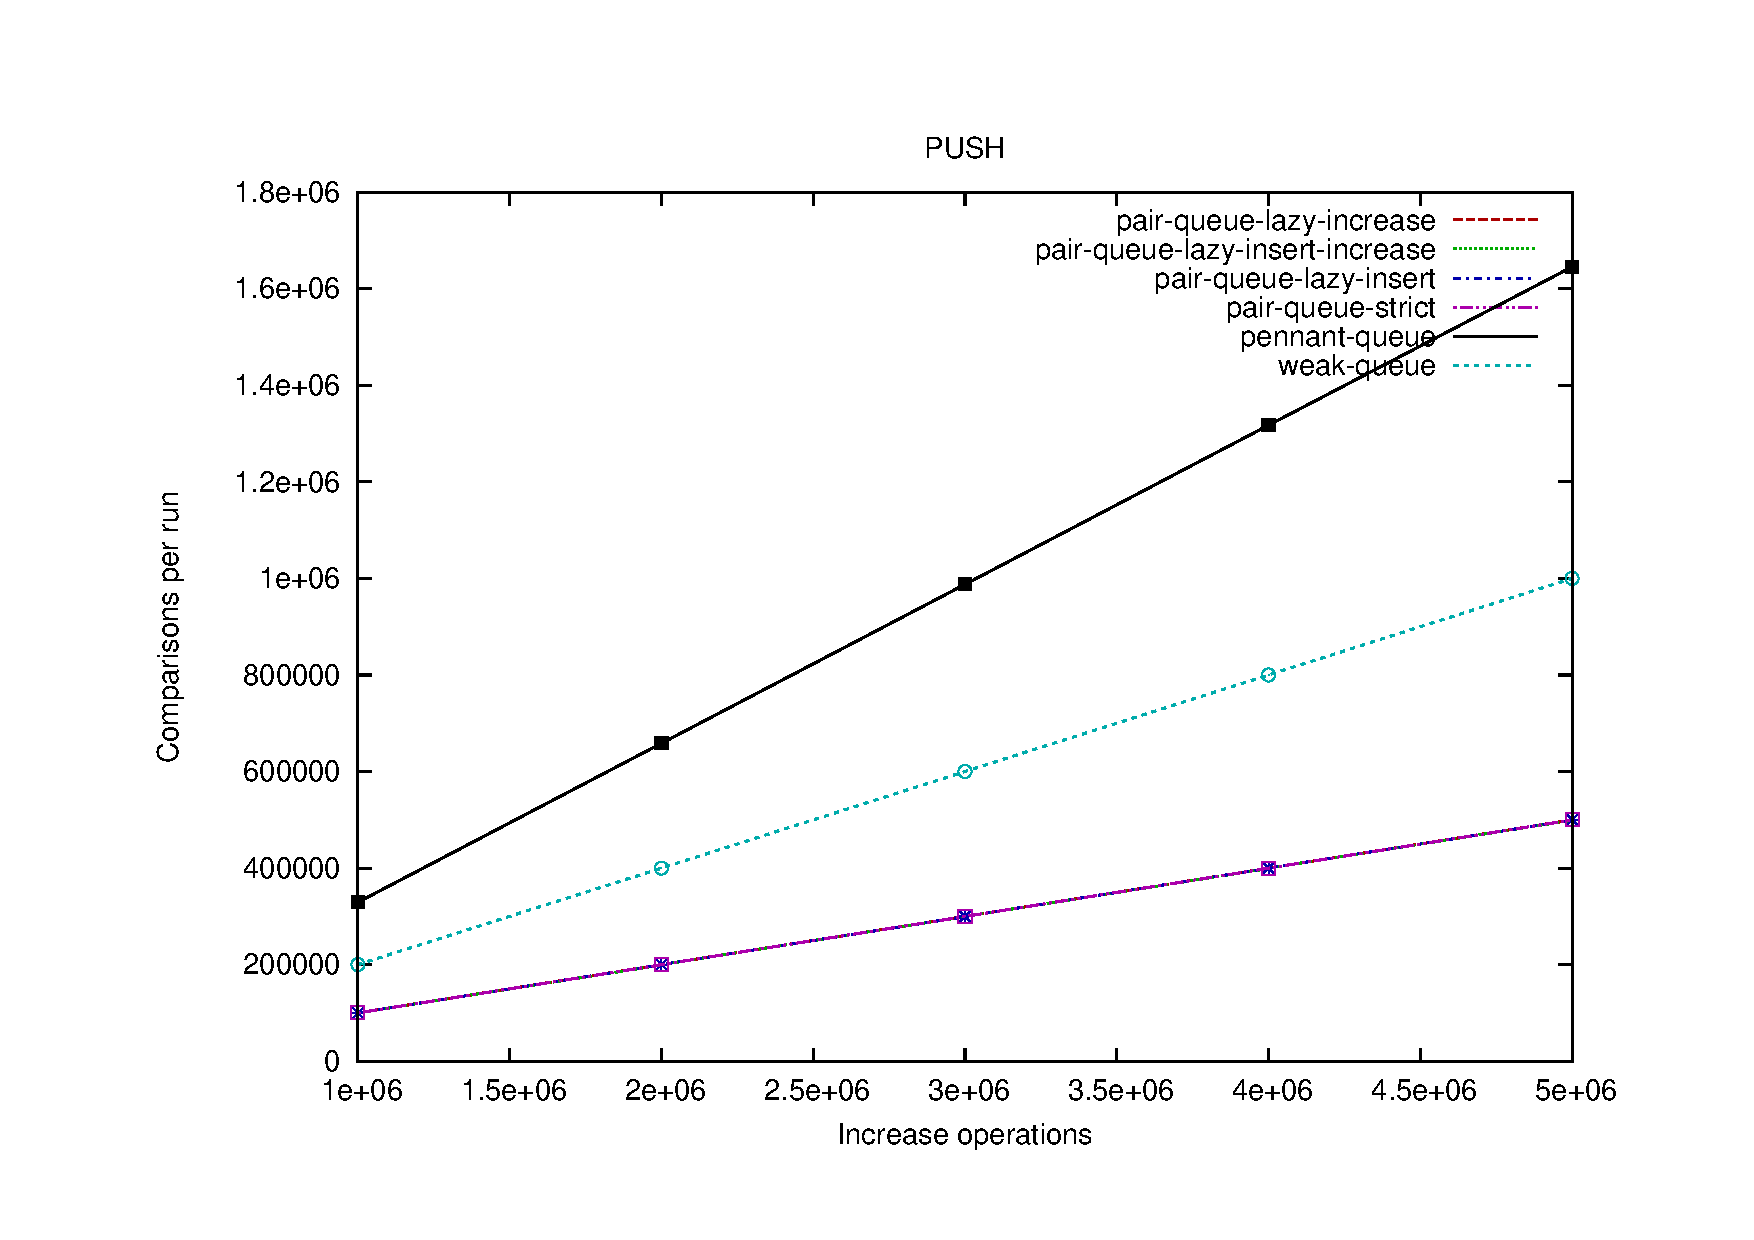
\includegraphics[width=.85\textwidth]{../graphs/push.pdf}
\end{frame}
\begin{frame}
\frametitle{Test: Pop}
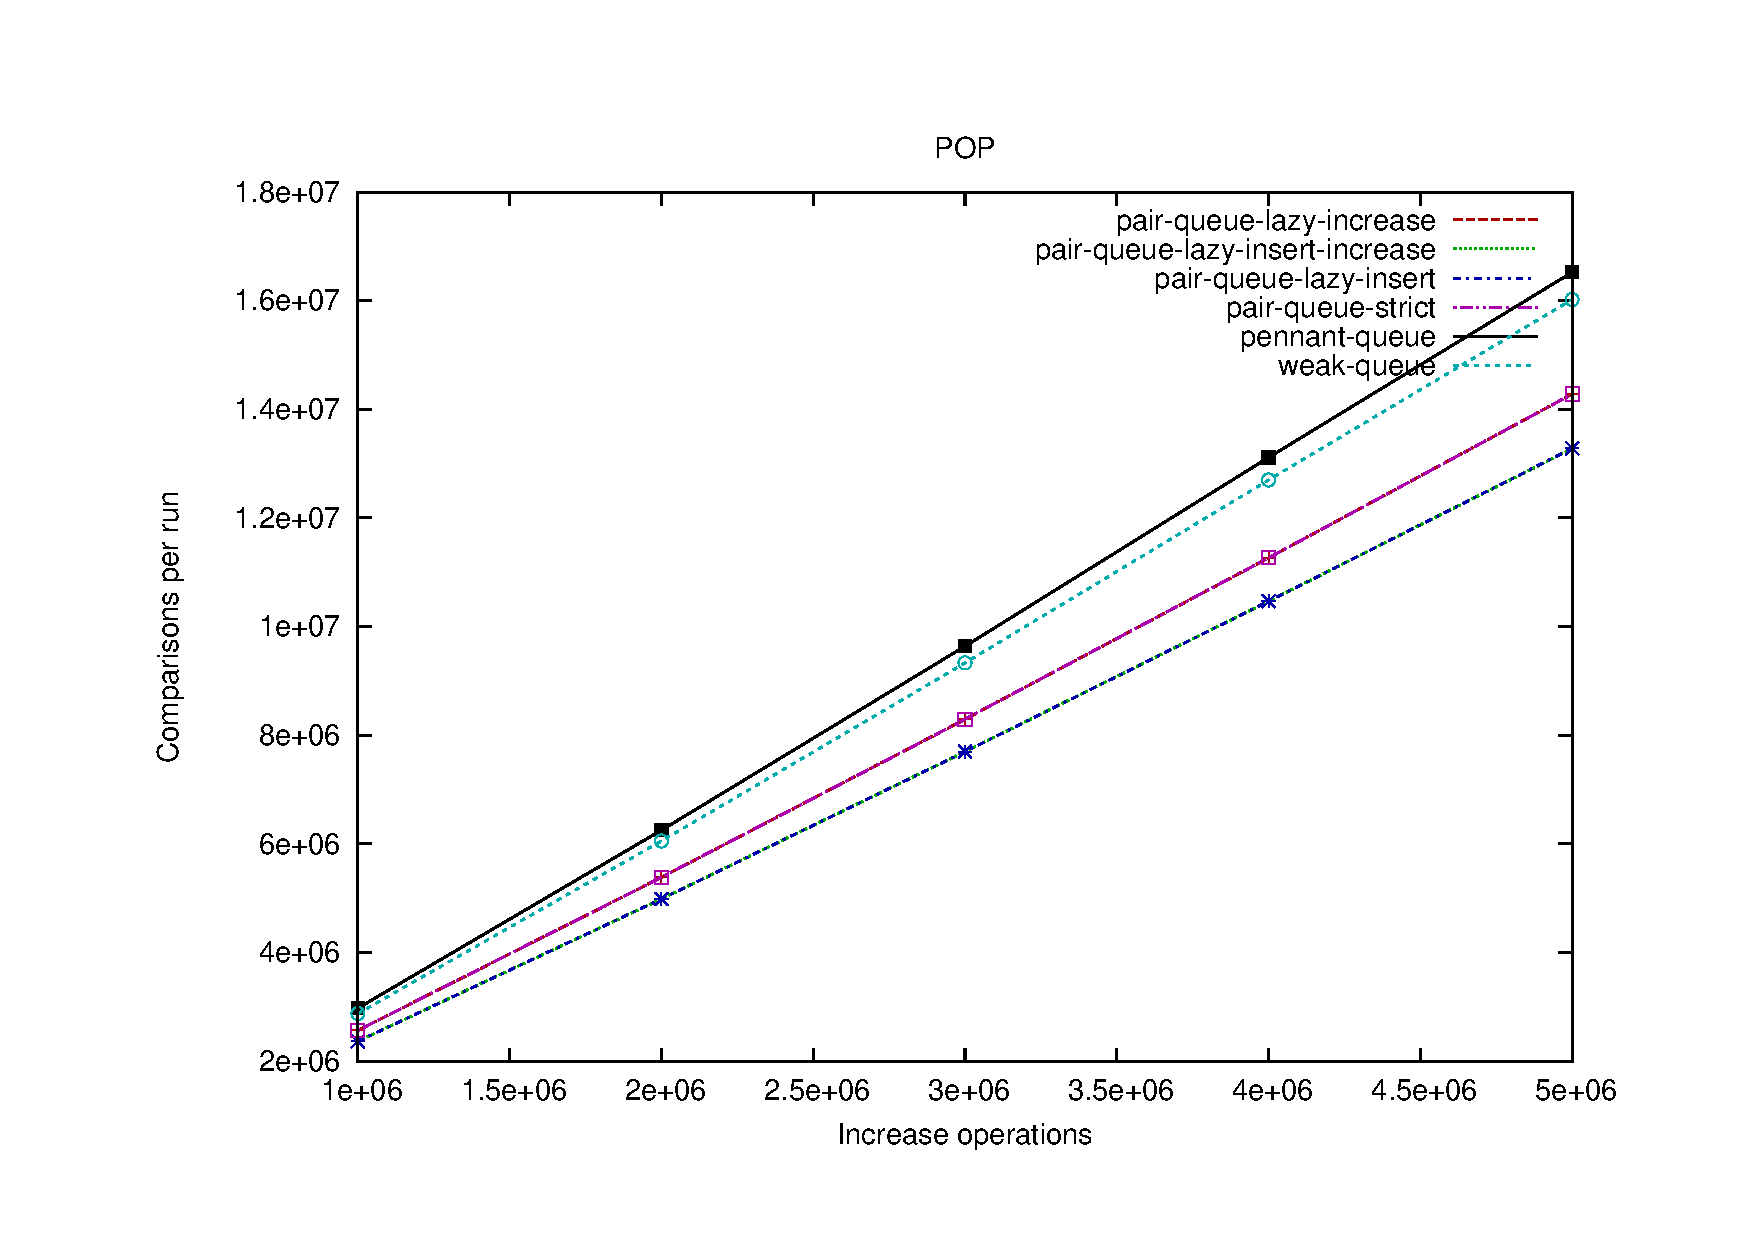
\includegraphics[width=.85\textwidth]{../graphs/pop.pdf}
\end{frame}
\begin{frame}
\frametitle{Test: Erase}
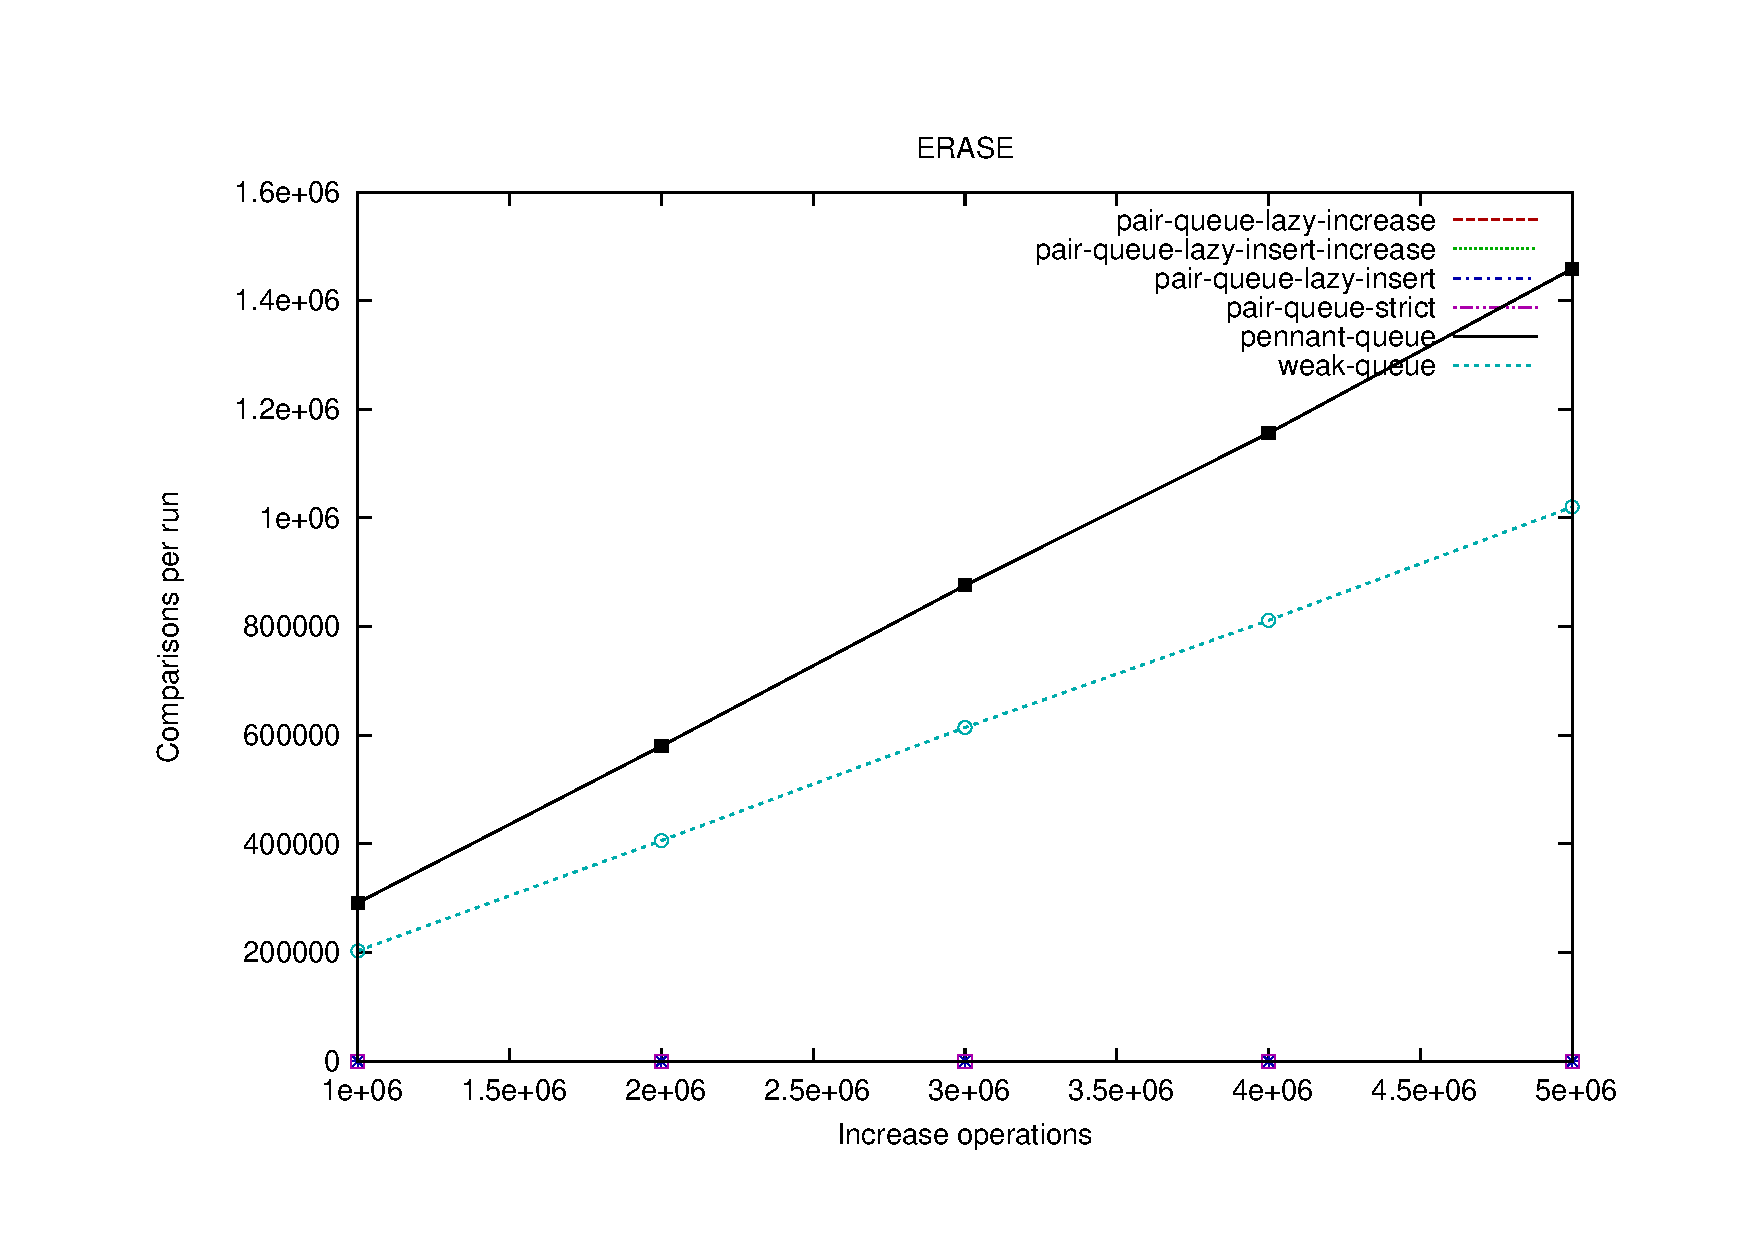
\includegraphics[width=.85\textwidth]{../graphs/erase.pdf}
\end{frame}
\begin{frame}
\frametitle{Test: Increase}
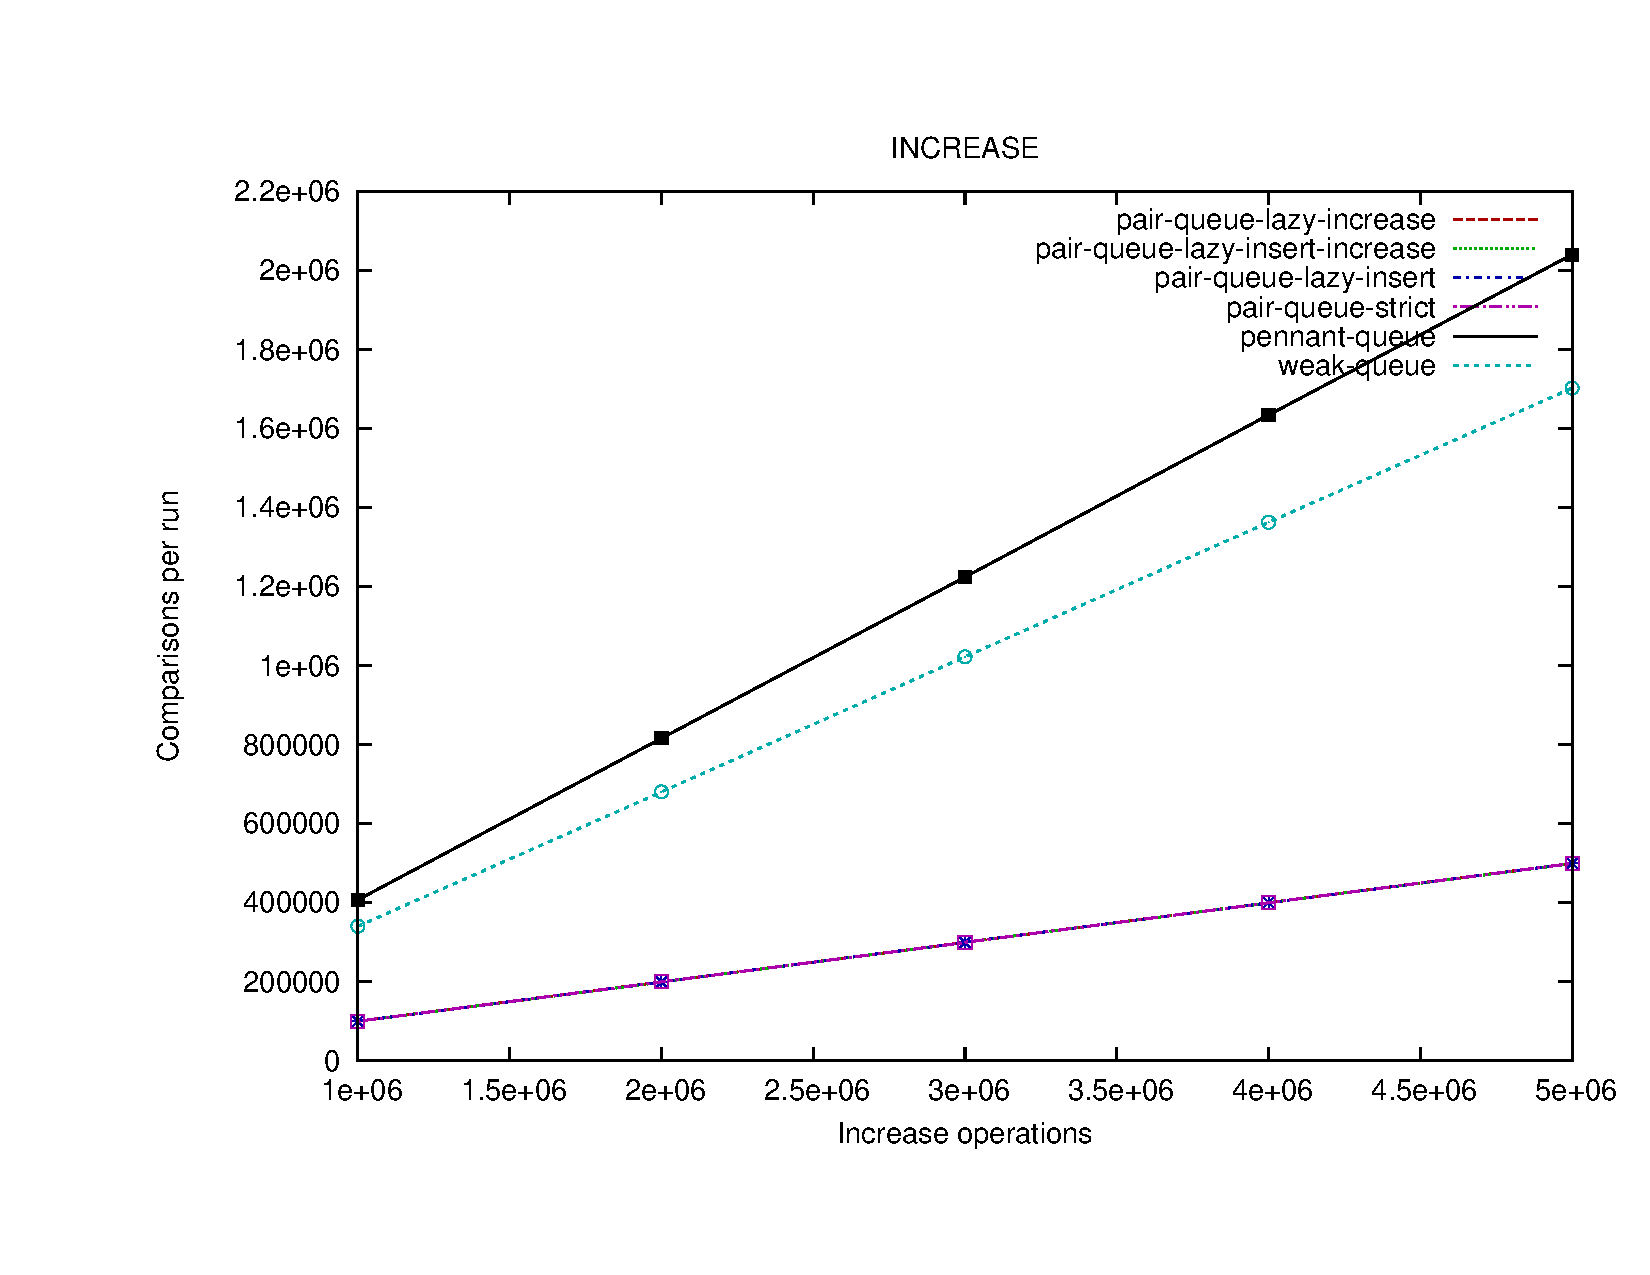
\includegraphics[width=.85\textwidth]{../graphs/increase.pdf}
\end{frame}
\begin{frame}
\frametitle{Test: Increase2}
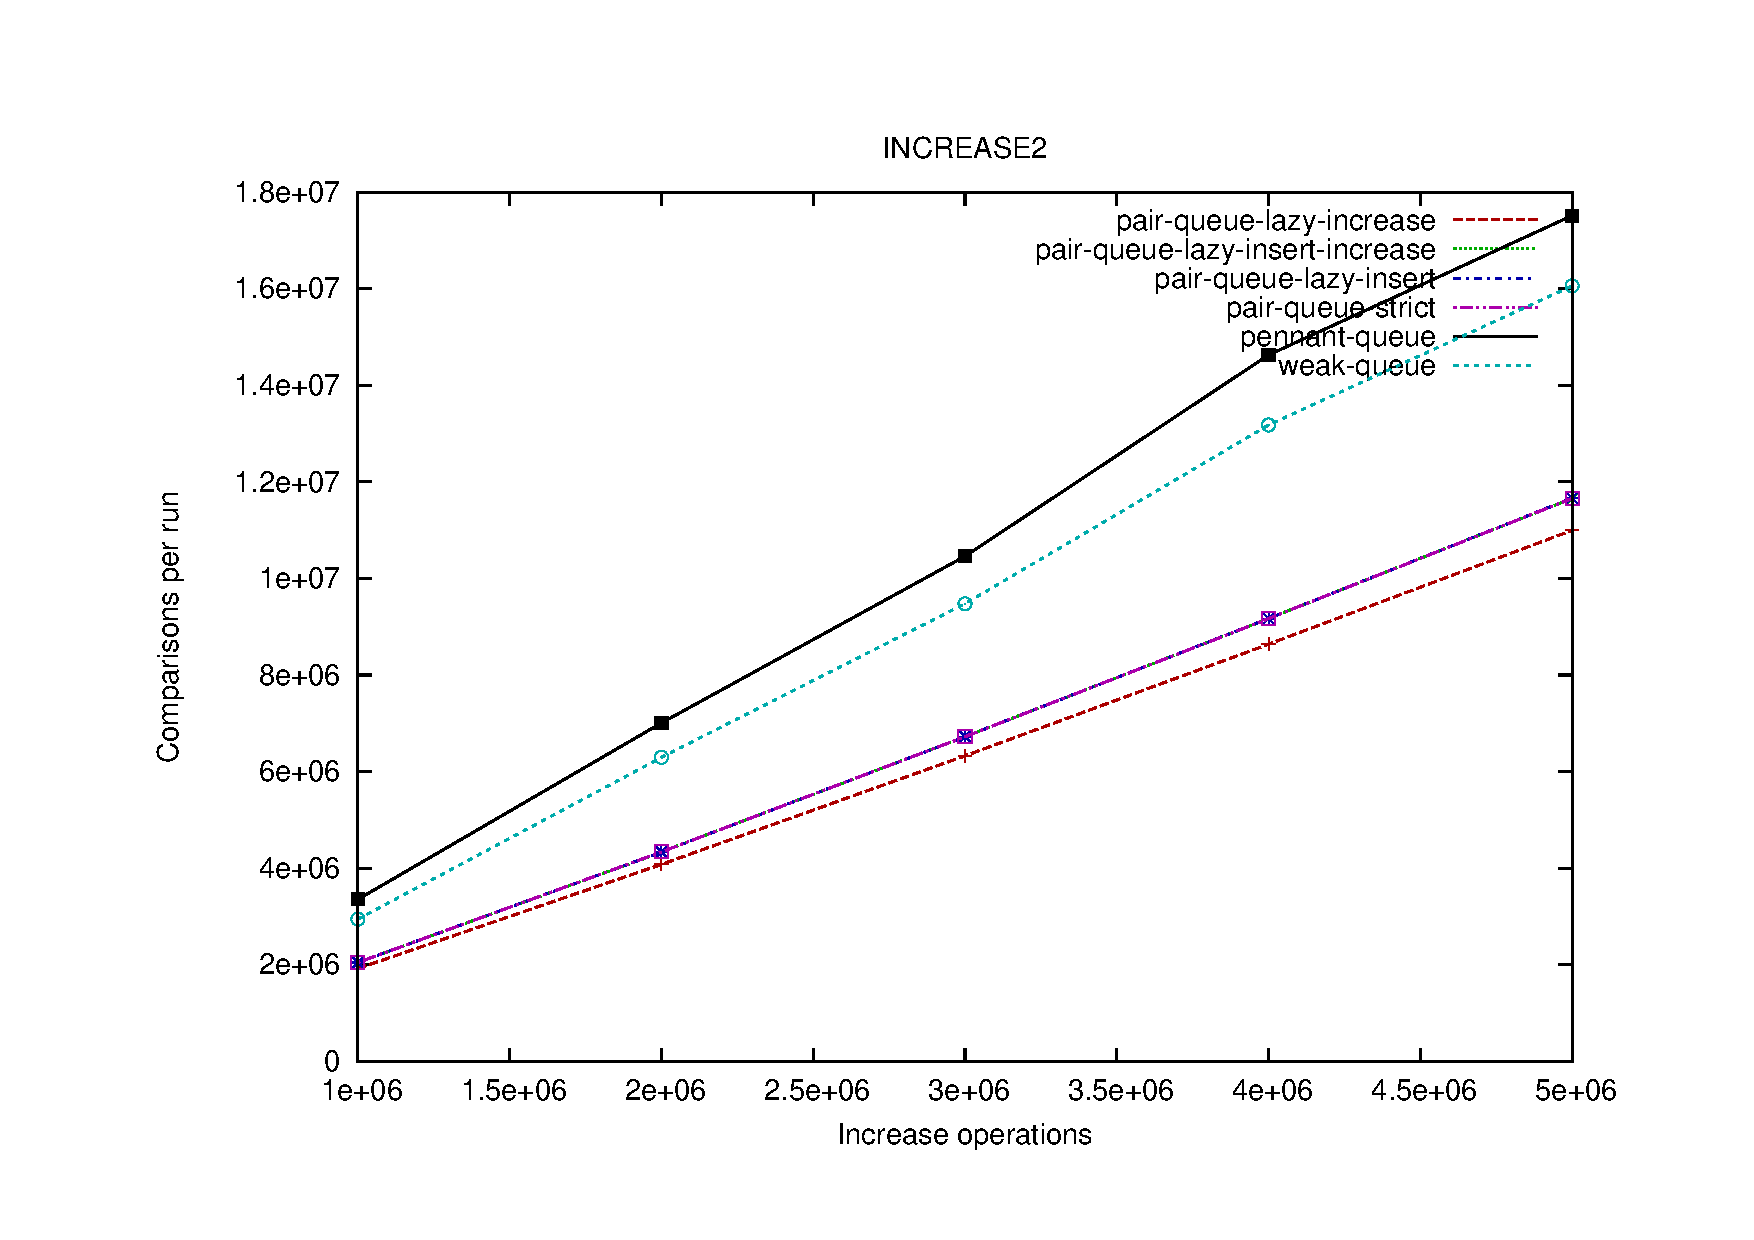
\includegraphics[width=.85\textwidth]{../graphs/increase2.pdf}
\end{frame}
\begin{frame}
\frametitle{Test: Increase3}
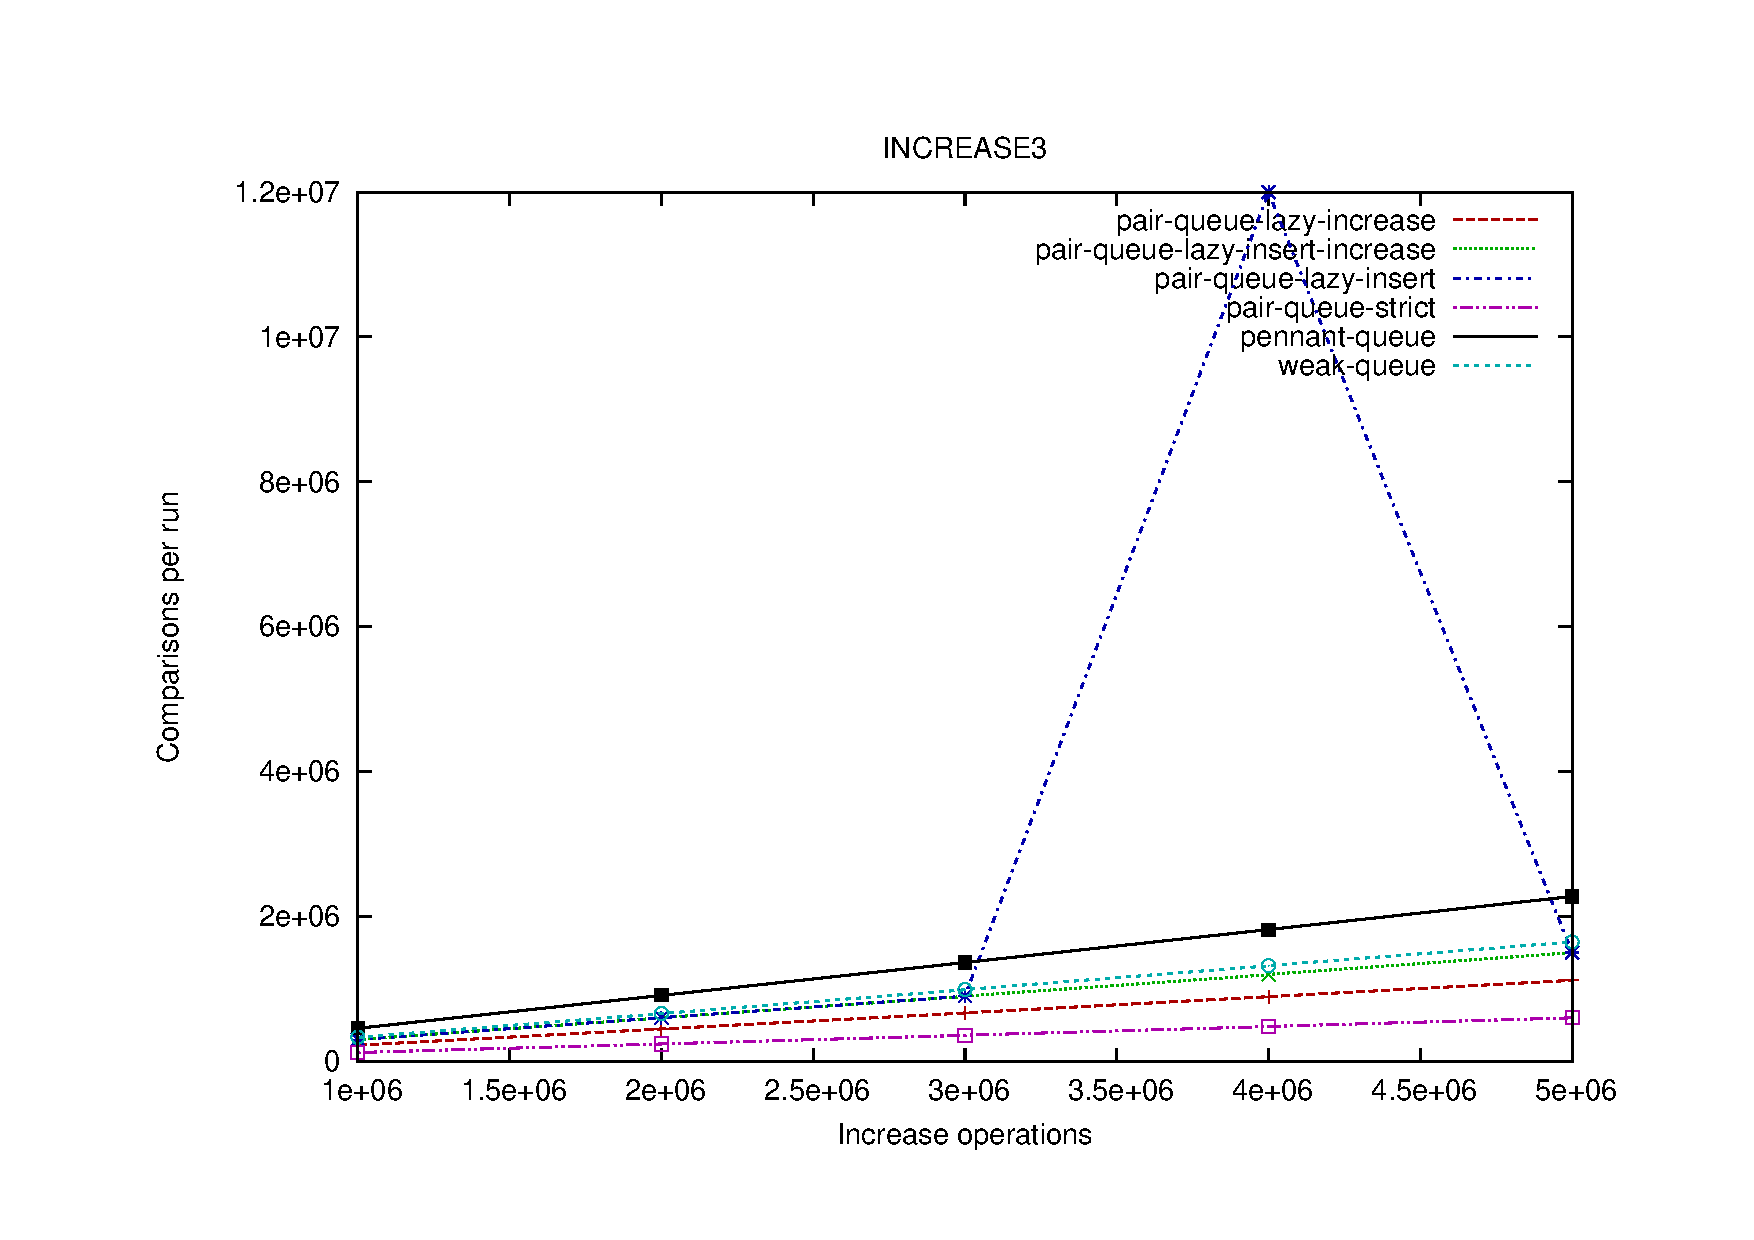
\includegraphics[width=.85\textwidth]{../graphs/increase3.pdf}
\end{frame}
\begin{frame}
\frametitle{Test: Increase4}
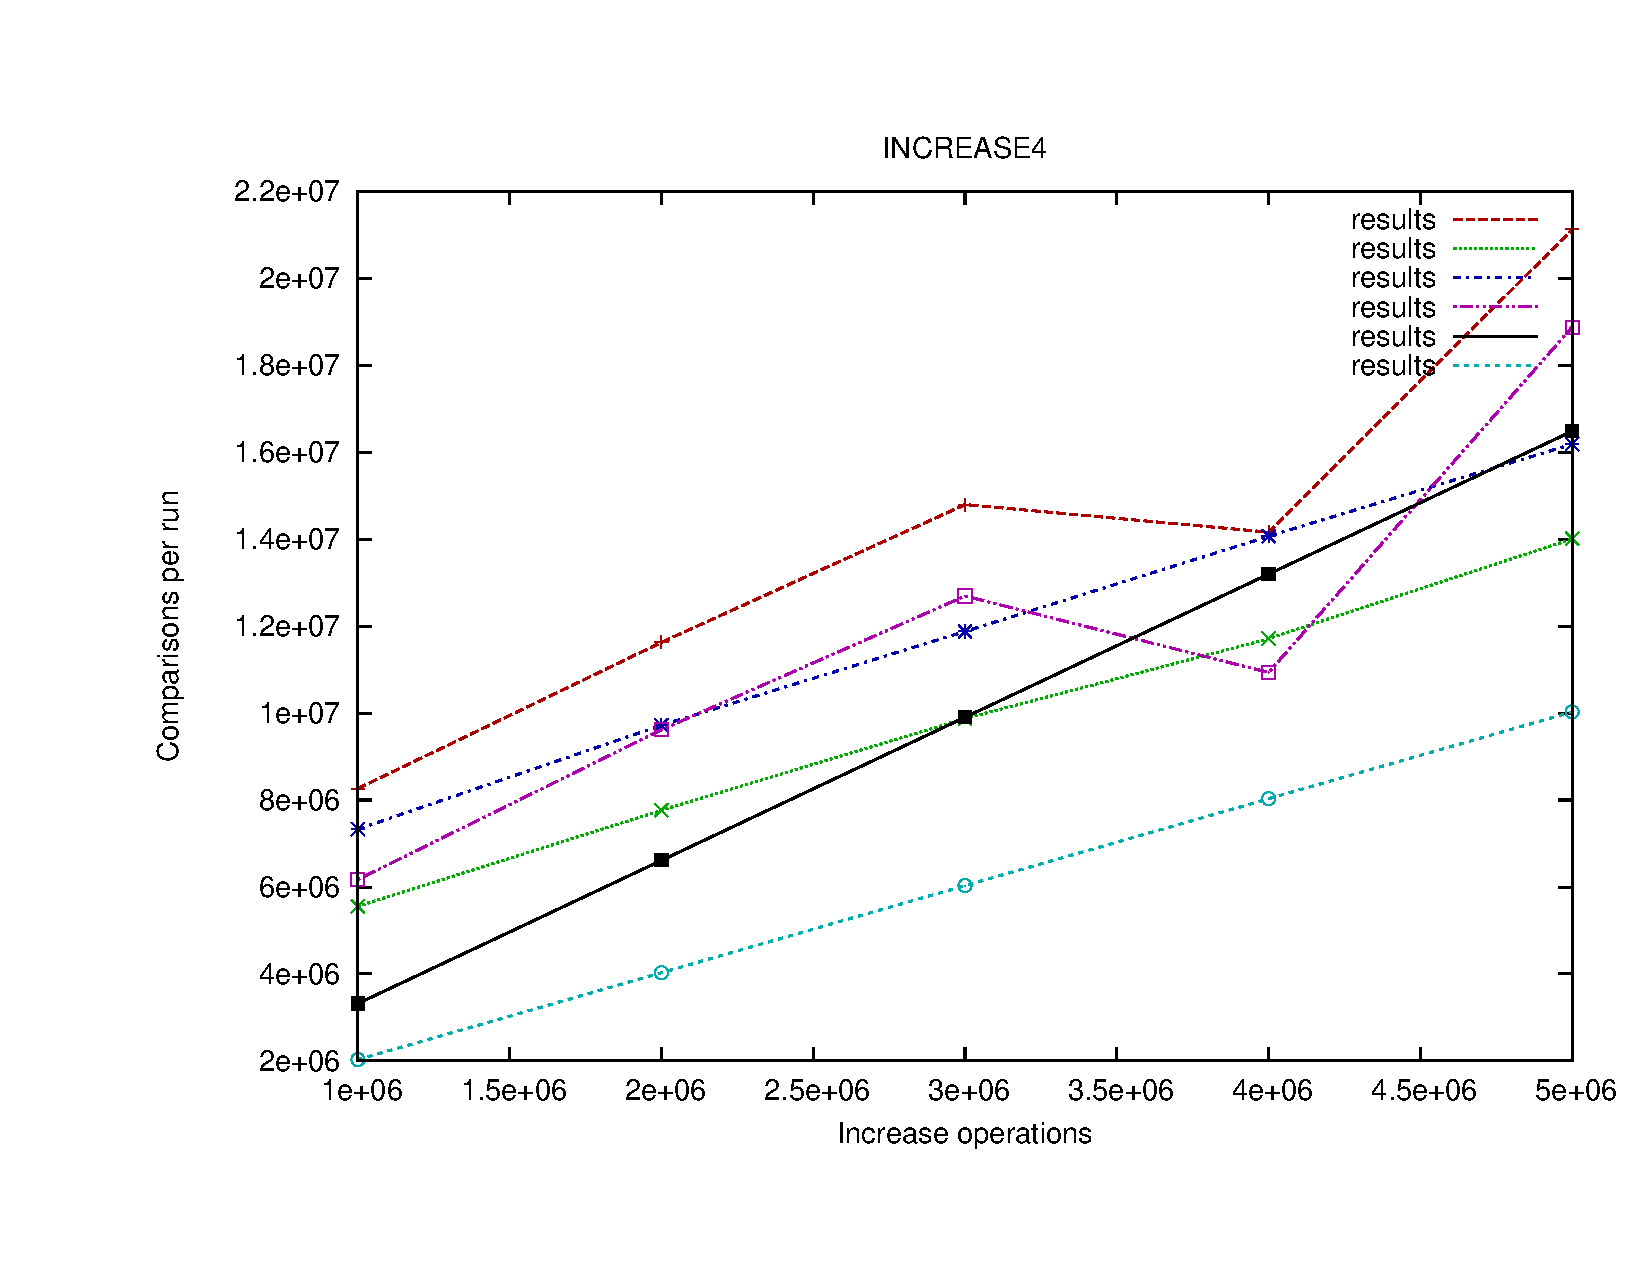
\includegraphics[width=.85\textwidth]{../graphs/increase4.pdf}
\end{frame}
\begin{frame}
\frametitle{Test: Dijkstra}
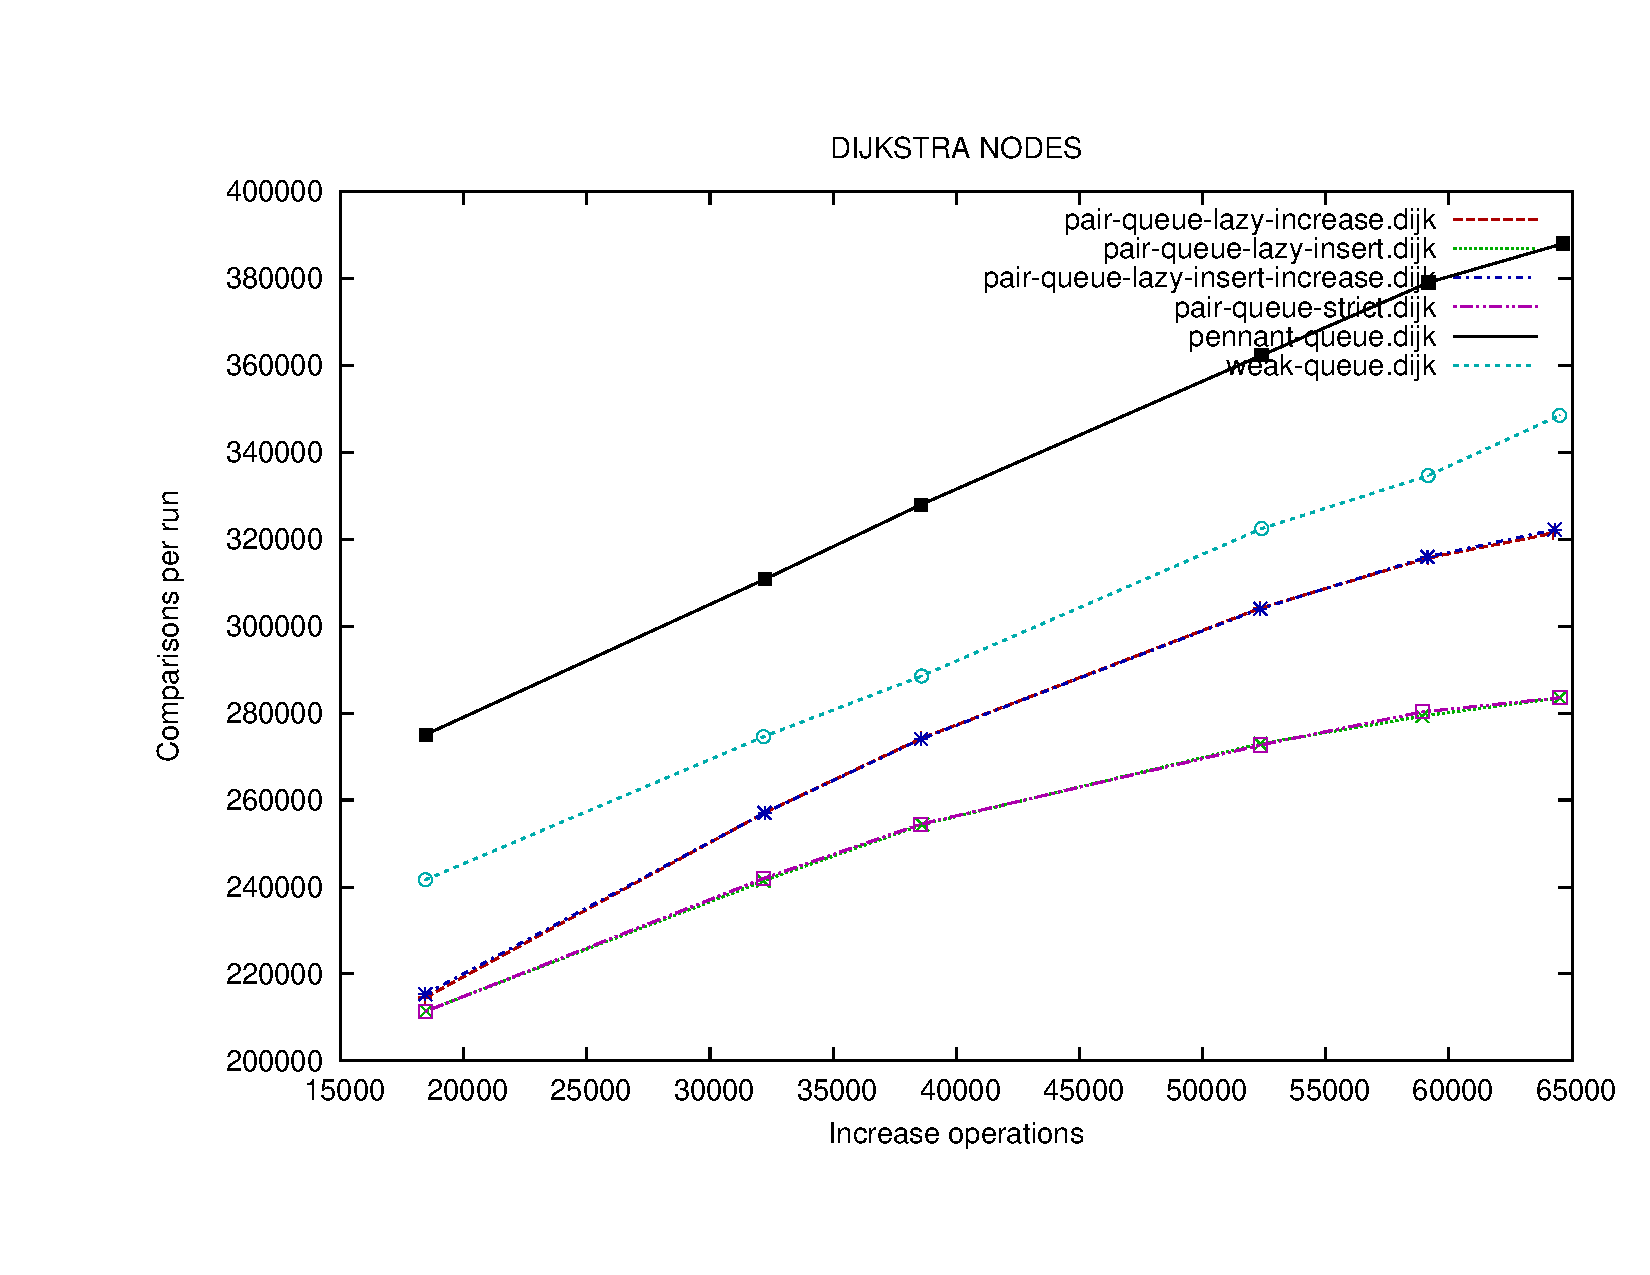
\includegraphics[width=.85\textwidth]{../graphs/dijk1.pdf}
\end{frame}
\begin{frame}
\frametitle{Test: Dijkstra}
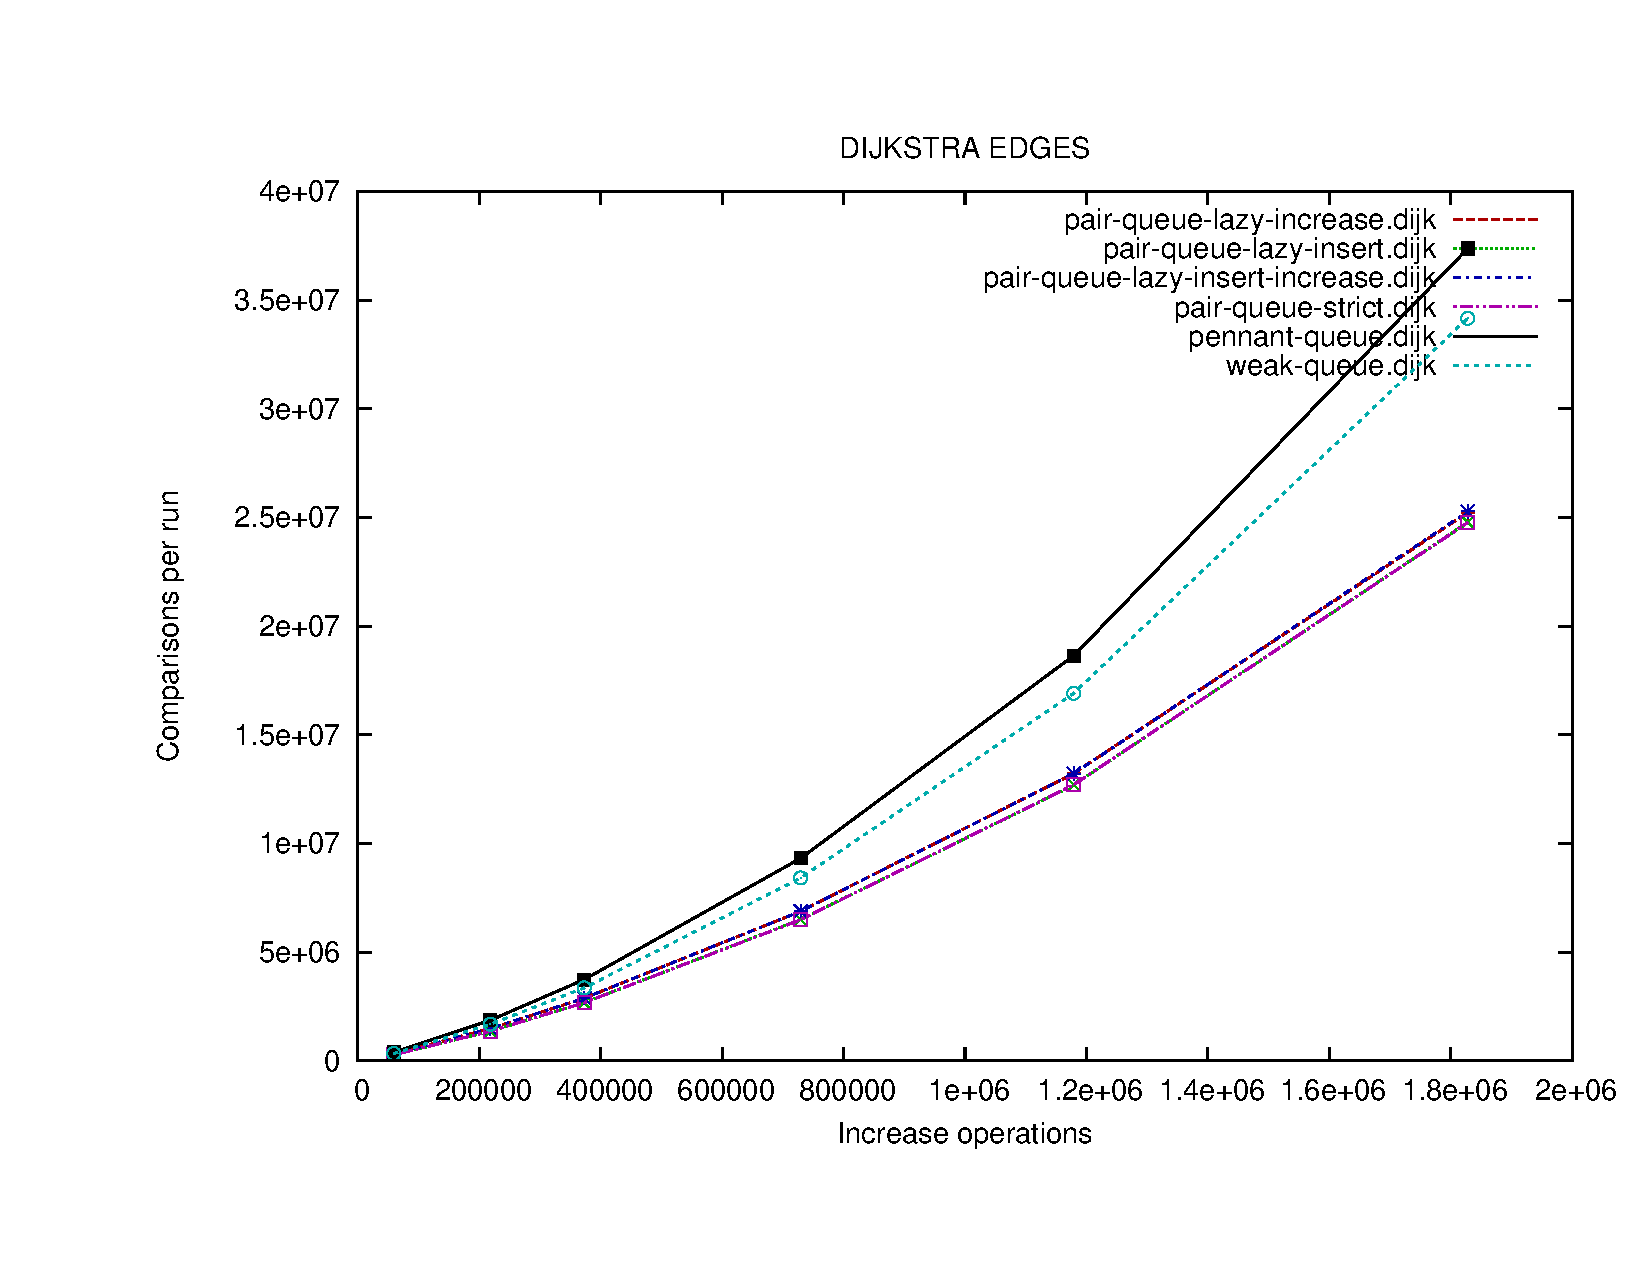
\includegraphics[width=.85\textwidth]{../graphs/dijk2.pdf}
\end{frame}

\begin{frame}


\subsection{Conclusion}
\frametitle{Conclusion}

\textbf{What we concluded:}
\begin{itemize}
\item Synthetic tests can be misleading
\item Pairing heaps are generally a well-performing structure
\item Variations of pairing heaps seems to perform equally
\end{itemize}

\textbf{Future work:}
\begin{itemize}
\item Better benchmarks
\item Larger instances
\item CPU-timings and profiling
\end{itemize}

\end{frame}


\end{document}

